\chapter{Multivariate extremes}
\label{sec:multivariate}
\section{Basic setup}

We will restrict ourselves to the two-dimensional case but some theorems and results will be stated for arbitrary $D$ dimensions. The $D$-simplex on which our considered distributions will be defined is the set
$$
S_D :=\left\{x \in \mathbb{R}^D_+ : \sum_{i=1}^D x_i = 1\right\}
$$

When $D=2$, that means that we only need to define a distribution on $ x_1 \in [0,1]$, and $x_2 = 1-x_1$ is completely determined by $x_1$. As mentioned in Section \ref{sec:intro}, we are going to consider distributions that are a mixture of $K$ beta distributions:

$$
\nu^*(x_1,x_2) = \prod_{k=1}^K \pi_k Beta(x_1;\alpha_k,\beta_k), \quad  0<x_1<1,
$$
with
$$
\prod_{k=1}^K \pi_k= 1, \quad \pi_k \geq 0 .
$$

The mean of this distribution is
$$
\mathbb{E}[X_1] = \sum_{k=1}^K \pi_k\frac{\alpha_k}{\alpha_k + \beta_k}, \hspace{10pt} (X_1,X_2) \sim \nu^*,
$$
But in general this is not equal to $1/2$ and so this class of distributions does not satisfy Theorem 8.1.
In section \ref{sec:tilting} we will see how to tilt a wide class of distributions to force the mean constraint $1/D$ to hold, and will apply it to our case.

\section{Construction of angular distributions}
\label{sec:tilting}
%using thm 2 of Coles and Tawn (1991)
%What I already have in this section plus simple explanation
%examples of simulation and tilting

The main tool for tilting distributions is Theorem 2 from the 1991 paper from Coles and Tawn \cite{ColesTawn}, which we state again here for completeness:\\


\begin{theorem}

If $h^*$ is any positive function on $S_D$ with finite first moments, then

$$
\nu(w) = (m^Tw)^{-(D+1)}D^{-1} \left( \prod_{d=1}^{D}m_d \right) \nu^*\left(\frac{m_1w_1}{m^Tw}, \ldots , \frac{m_Dw_D}{m^Tw}\right),
\quad (w_1,\ldots,w_D) \in S_D,
$$
where
$$
m_d = \int_{S_D} u_d\nu^*(u)du, \quad d=1, \ldots ,D,
$$
satisfies mean constraints $1/D$ and is therefore the density of a valid measure function $\nu$.

\end{theorem}

To verify that the theorem holds, we need to verify that the Jacobian of the transformation

$$
W_d = \dfrac{W^*_d/m_d}{\sum_{c=1}^{D}W_c^*/m_c},\hspace{10pt}
W_d^* = \frac{m_dW_d}{\sum_{c=1}^{D}m_cW_c},\hspace{10pt}
d=1,\ldots,D,
$$
is $|\partial w^*/\partial w | = (m^Tw)^{-D} \prod_{d=1}^{D}m_d$.
To do this, we rewrite the first transformation as

$$
w_s^* = \frac{m_dw_d}{m_D+\sum_{c=1}^{D-1}(m_c - m_D)w_c}, \hspace{10pt}
d=1,\ldots,D-1.
$$
by noting that $w=(w_1,\ldots,w_D) \in S_D$. To simplify notation, we write
$m^Tw = m_D + \sum_{c=1}^{D-1}(m_c - m_D)w_c$. As such,

\begin{align*}
\partial w_d^*/\partial w_d &= m_d/(m^Tw) - m_dw_d(m_d - m_D)/(m^Tw)^2 , \\
\partial w_d^*/\partial w_c &= - m_dw_d (m_c - m_D)/(m^Tw)^2, \quad c\neq d.
\end{align*}

This defines a matrix that we can write as $A + ab^T$, where

\begin{align*}
A &= {\rm diag}(m_1,\ldots,m_{D-1})/(m^Tw) , \\
a &= (m_1w_1,\ldots,m_{D-1}w_{D-1})^T , \\
b &= -(m_1 - m_D,\ldots,m_{D-1} - m_D)^T/(m^Tw)^2.
\end{align*}


Let's recall the determinant lemma:
Let $A$ be an invertible $ p \times p $ matrix, and let $a,b,$ be vectors of length $p$.
Then $|A + ab^T| = |A|(1 + b^TA^{-1}a)$. \\

In our case, $A$ is diagonal, so
\begin{align*}
|A| &= (m^Tw)^{-(D-1)} \prod_{c=1}^{D-1}m_c , \\
b^TA^{-1}a &= -\frac{m^Tw + m_D}{m^Tw},
\end{align*}
so 
$$1 + b^TA^{-1}a = m_D/m^Tw.$$

Therefore, $|\partial w^*/\partial w| = (m^Tw)^{-D} \prod_{d=1}^Dm_d$, so the variable $W=(W_1,\ldots,W_D)$ has the probability density function
$$
f(w) = (m^Tw)^{-D} \left(\prod_{d=1}^D m_d\right) \nu^* \left(\frac{m_1w_1}{m^Tw},\ldots,\frac{m_Dw_D}{m^Tw}\right)
$$
For every $d$, $W_d^*/m_d$ has unit expectation, which leads to the following equality
$$
1 = \mathbb{E} \left( \frac{W_d^*}{m_d} \right) = \mathbb{E} \left( \frac{W_d}{m^TW} \right)
= \int_{S_{D-1}} w_d (m^Tw)^{-(D+1)} \left(\prod^D_{d=1} m_d \right) \nu^* \left(\frac{m_1w_1}{m^Tw},\ldots,\frac{m_Dw_D}{m^Tw}\right) {\rm d}w
$$
by noting that $\sum_d w_d = 1$ and summing the previous equality over $d$, we get that
$$
\nu (w) = D^{-1}(m^Tw)^{-(D+1)} \left(\prod_{d=1}^D m_d\right) \nu^* \left(\frac{m_1w_1}{m^Tw},\ldots,\frac{m_Dw_D}{m^Tw}\right).
$$
which is a well defined density on $S_{D-1}$ satisfying the mean constraint
$$
\int_{S_{D-1}} w_d \nu (w) {\rm d}w = D^{-1}, \quad d=1,\ldots,D.
$$

\begin{figure}[h]
\centering
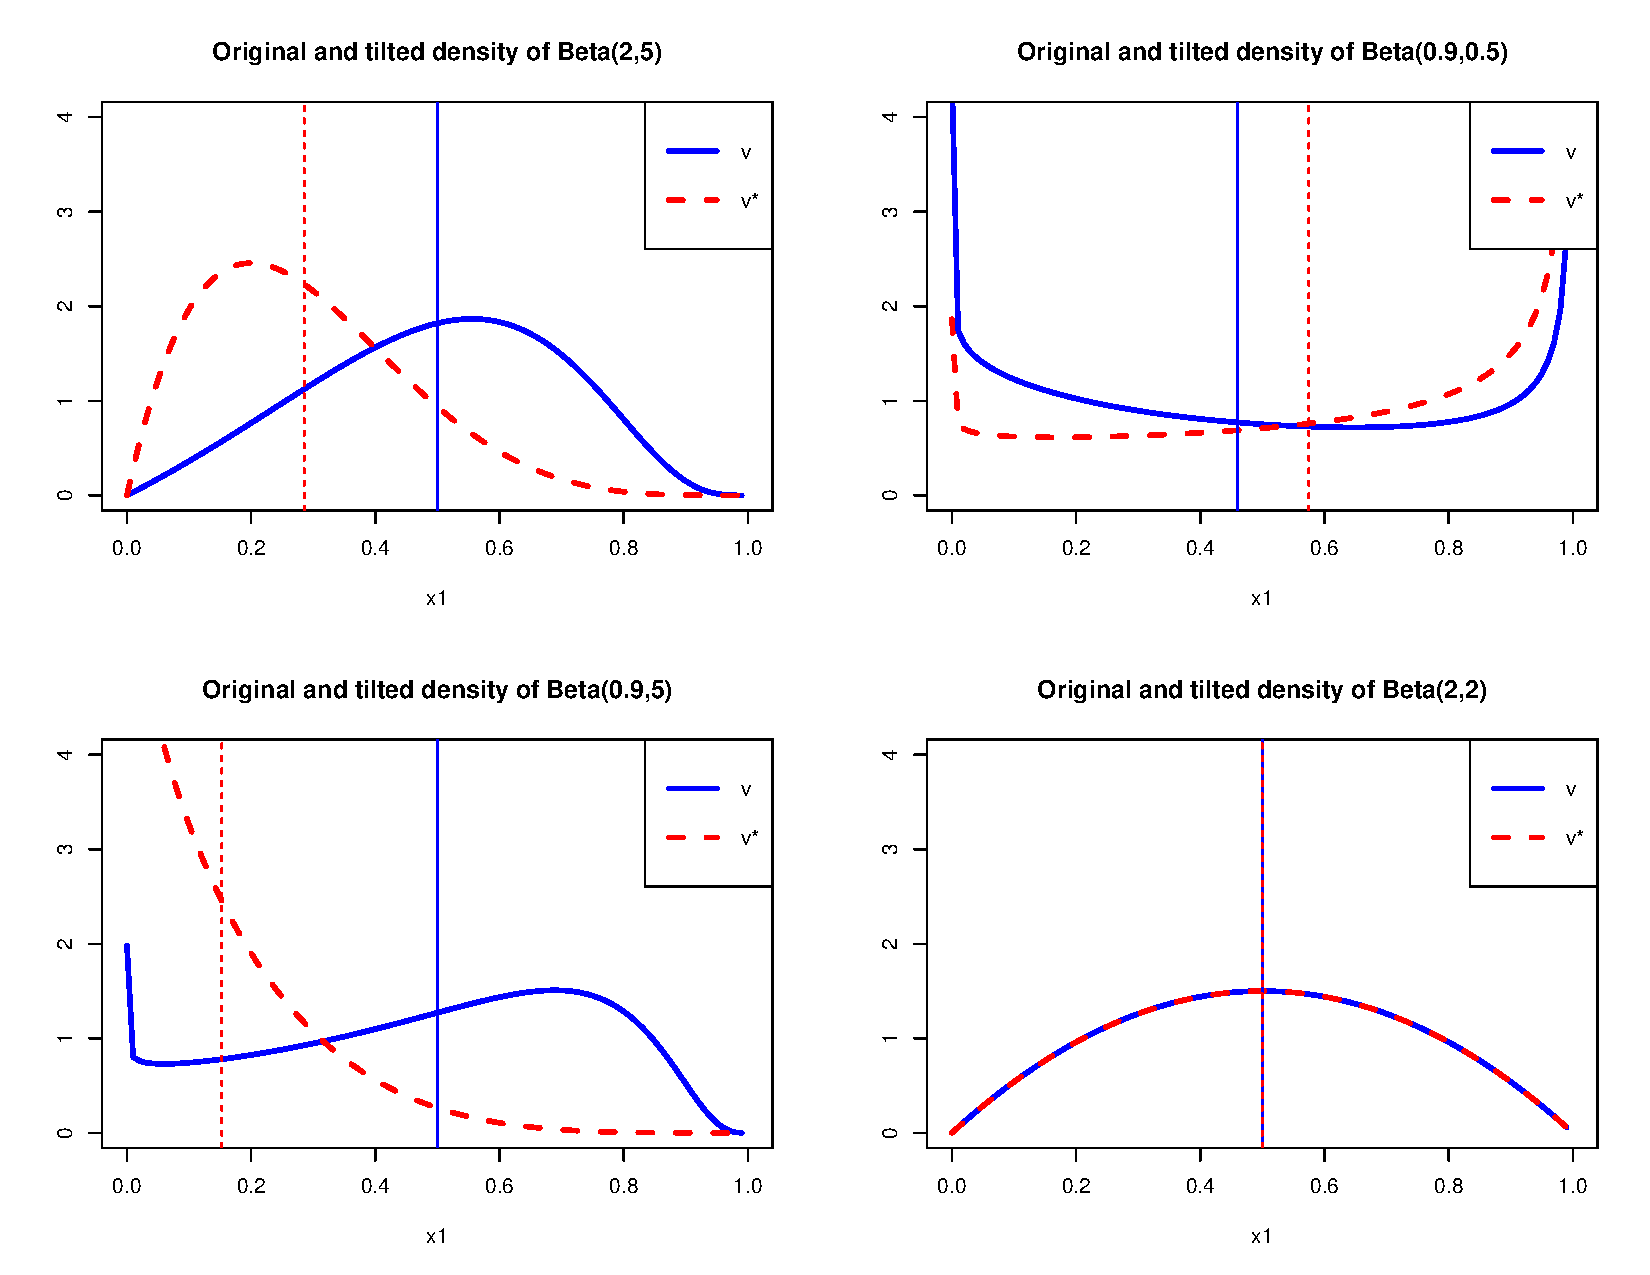
\includegraphics[width=\textwidth]{density_tilt.pdf}
\caption{Graphs of beta distributions for various shape parameters, before and after tilting. The vertical lines represent the means. As we can see, although the original densities have various means, the tilted densities all have mean 0.5, and when the original distribution already has the correct mean, it is not tilted.}
\label{fig:density_tilt}
\end{figure}

\subsubsection{Sampling from tilted density}
As we have seen in the proof of theorem 2, to construct the appropriate density $\nu$, we start with a density $\nu^*$, apply a change of variable to it, then tilt the result by diving it by $Dm^Tw$, which is bounded, in order to sample from the tilted density, we can sample from the original density $\nu^*$, transform the the samples, then apply the following Acceptance-Rejection step:

$$
U\leq m_{\min}/m^Tw
$$
where $m_{\min} = \min_d m_d$

This is because a realisation $W^*$ of $\nu^*$ that has been transformed has density $f$ and not $\nu$. But $m_{\min}/m^TW \leq 1$, so conditional on $W=w$ the event $U \leq m_{\min} /m^Tw$ has probability $m_{\min}/m^Tw$. Thus the marginal density of the $W$ for which the event occurs is proportional to $f(w)/(m^Tw)$ and has to be $\nu$.

The acceptance probability is given by
$$
\int \frac{m_{\min}}{m^Tw}f(w){\rm d}w = Dm_{\min} \int \nu (w) {\rm d} w = Dm_{\min}
$$

Thus the number of accepted samples is proportional to $m_{min}$, so the algorithm is the most efficient when all the $m_d$ are equal to $1/D$ which would mean our original density $\nu^*$ already satisfies the criteria and we would not have to run the algorithm at all.

\subsubsection{Tests}
Figure \ref{fig:historam_tilt} some examples of tilted mixtures of beta distributions, sampled using the algorithm, and the theoretical tilted distributions using the formula.

\begin{figure}[h]
\centering
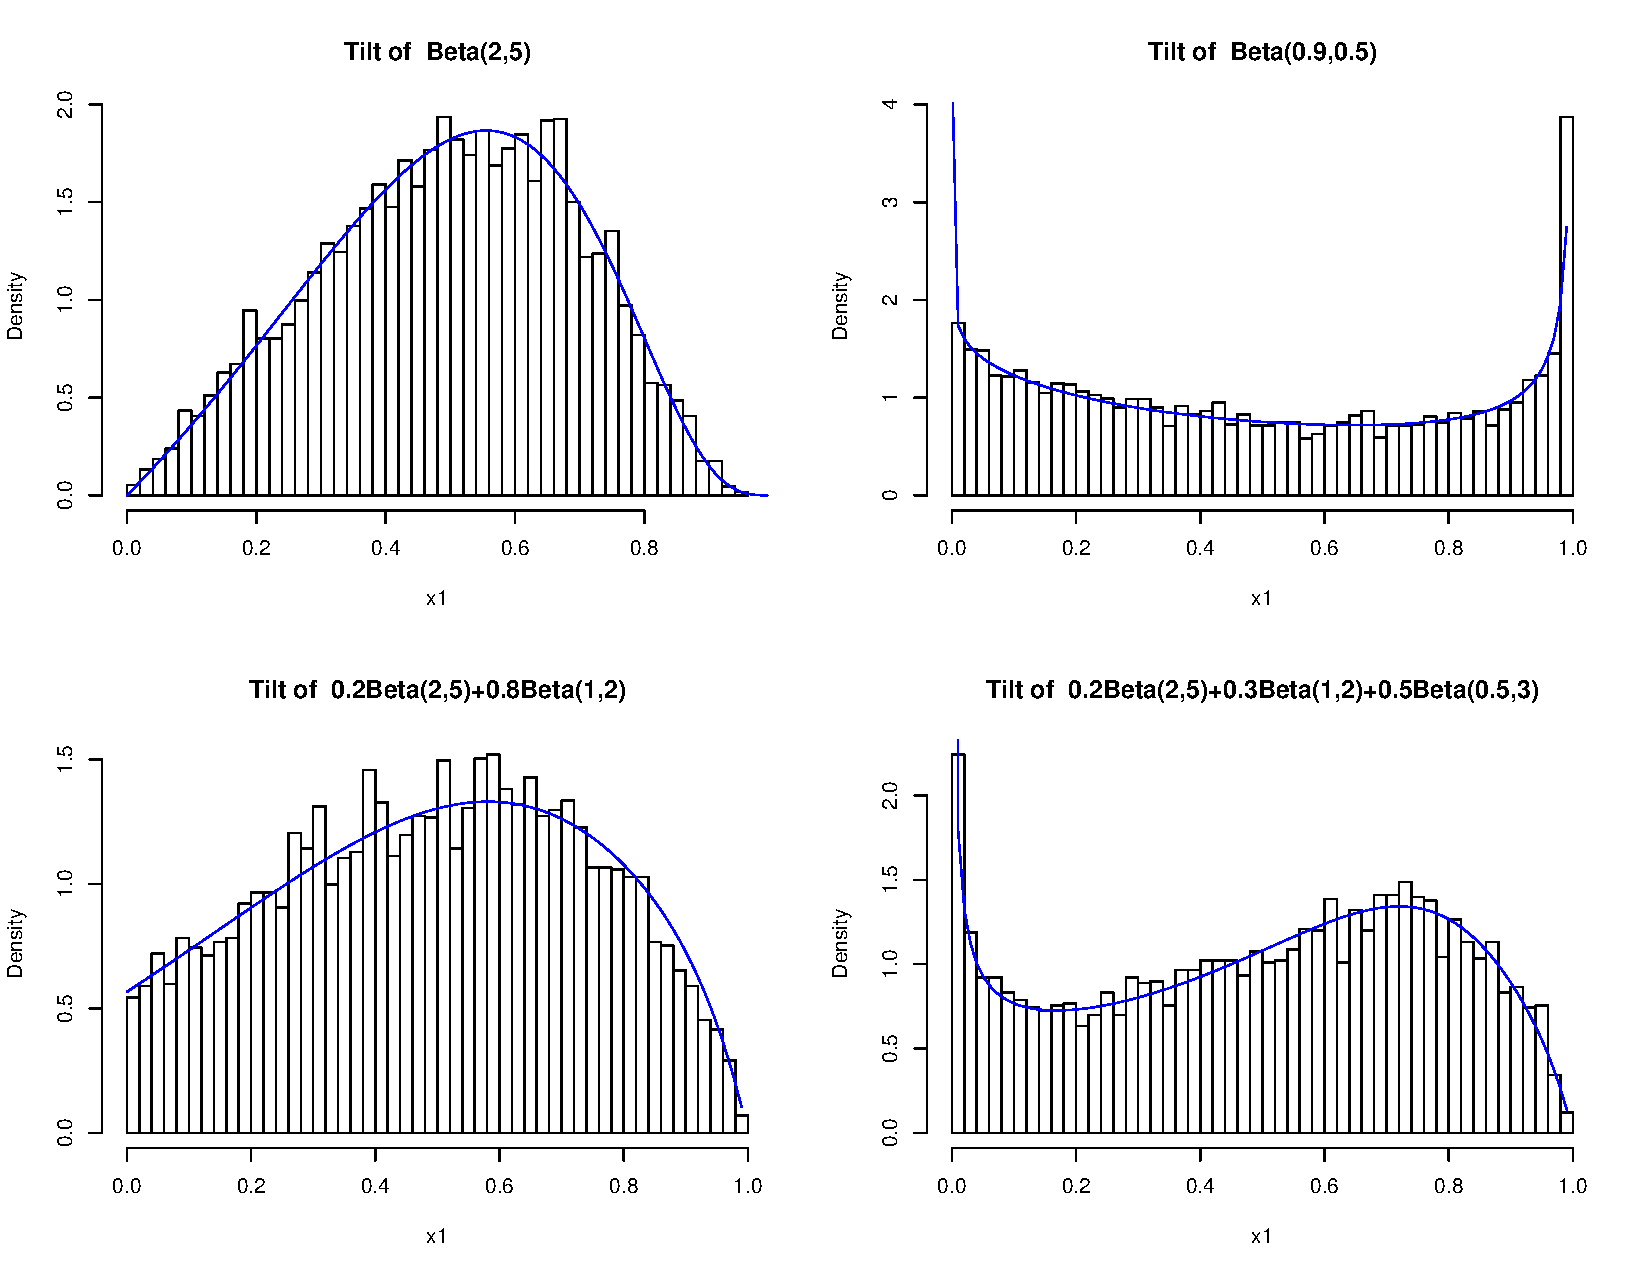
\includegraphics[width=\textwidth]{histogram_tilt.pdf}
\caption{Histograms of $10^4$ samples from various mixtures of beta distributions that have been tilted. The pdfs of the distributions are overlaid in blue. As we can see, the sampling algorithm for the tilted mixtures is correct.}
\label{fig:historam_tilt}
\end{figure}




\section{Tilted mixtures are dense}
%if possible, show that the class of tilted mixture distributions is dense in the class of distributions with mean 1/D (analogous to Appendix in Boldi and Davison)

To prove that the set of all tilted distributions are dense within the class of all distributions on the $p$-dimensional simplex $S_p$ which satisfy the mean constraint $\mu=p^{-1} {\rm \textbf{1}}_p$, where ${\rm \textbf{1}}_p$ is the unit vector in $\mathbb{R}^p$.

Boldi and Davison prove in appendix A of \cite{BoldiDavison} that the class of Dirichlet mixtures that satisfy the mean constraint are weakly dense. From there we may simply remark that a Dirichlet mixtures that satisfy the constraint is itself tilted and thus belongs to the class of all tilted distributions.
The final step is to remark that if a subclass of the tilted distributions is already weakly dense, then the whole class is therefore weakly dense as well.